\documentclass{article}
\usepackage[margin=1in]{geometry} 
\usepackage{amsmath,amsthm,amssymb,amsfonts, fancyhdr, color, comment, graphicx, environ}
\usepackage{xcolor}
\usepackage{mdframed}
\usepackage[shortlabels]{enumitem}
\usepackage{indentfirst}
\usepackage{hyperref}
\hypersetup{
    colorlinks=true,
    linkcolor=blue,
    filecolor=magenta,      
    urlcolor=blue,
}
\usepackage{pgfplots}
\pgfplotsset{width=10cm,compat=1.9}
\pgfplotsset{compat=1.17}
\usepackage{tikz}
\usepackage{caption}

\setlength{\parindent}{0pt}


%for headers 
\pagestyle{fancy}
\fancyhf{} % for header/footer

\lhead{Creel}
\rhead{ENV 795 - Nature as Capital}
\chead{\textbf{Conceptual Models}}

\title{Week 1 -- Conceptual Models}
\author{Andie Creel for Nature as Capital}
\date{January 30th, 2023}


\begin{document}
\maketitle

\section{Introduction -- 1/30/23}

\subsection{Course Objectives}

\begin{itemize}
    \item Apply capital theory to ecological systems
    \item Know when someone's model is BS
    \item People's attitude about models: skeptical, then learn how to do them and think of them as gospel, then move on to recognizing they're a simplifcation of reality that's also a very helpful tool 
\end{itemize}

\subsection{Never been a better time to study Natural Capital}

\begin{itemize}
    \item The economics of biodivesity: The Dasgupta Review
    \item UN's SEEA
    \item US's National Strategy to develop statistics for environmental economic decisions 
\end{itemize}

\subsection{The Issue}
Historically, ecological assets were plentiful. Society drew down ecological assets to build other forms of welath (human and produced). Markets allocate assets through price structure. Markets for the most part do a back job pricing capital assets. Markets do insanely bad at pricing natural assets. Allocation of assets is a mix of markets and non-market mechanisms. \\

We also need to keep clear positive and what is normative. \\

We are concerned with: sustainability and well-being (welfare). \\

We need to notice that investment and conservation are extremely similar, both about making decisions today to achieve a specific state of the world. Historically, conservation has been reactive but in this class we'll learn how to do conservation in a forward looking way. 

\subsection{Ecological Assets}
Ecology is the study of structure and function of living and nonliving things. \\

Function (flow) -- ecosystem services \\

Structure (stock) -- things we can measure and quantify, how many fish, how many tress. \textbf{Units of natural capital are ecological structures (or other natural resources).}

\subsection{Ecosystem Services}
The focus of ecosystem services is misplaced. There is nothing we do that doesn't include ecosystem services. A more disciplined way to think about the wealth provided by nature is as a capital asset, rather than trying to measure all the services provide by nature. 

\subsection{Natural Capital}
A capital asset stores wealth for the future. \\

Think of consumption as "enjoyment" rather than using something up. \\

Concept of natural capital is old. \\

"If expenditure is made with he intention of increasing future rather than current consumption, then it (the stock) should be treated as capital" Hulten (2006) \\

The Nature of Capital and Income, Irving (1906) -- income that doesn't flow through the cash door. \\\

"The nation behaves well if it treats the natural resources as assets which it must turn over to the next generation increase, and not impaired, in value." Roosevelt, speech to Colorado livestock associate, Denver, Aug. 29, 1910. \\

\subsection{Scarcity}
Prices and quantities are two difference side of the same coin. Concept of scarcity marries those. \\

Scarcity -- availability relative to demand of the relative opportunity cost of converting capital now. Different than a physical measure of quantity because it gets into demand. Do we want more?? \\

"We are using natural capital because it is valuable; the reason we are losing natural capital is it is free." Ed Barbier \\

\subsection{Models}
We need models to clarify thinking of management, clarify hypothesis for science, better understand/communicate our understanding of complex systems. It's useful to understand how simple things really are. \\

Most models are built off very simple building blocks. However, they require you to be very clear in your thinking. Reality is incredibly complex, beyond comprehension. But models can simplify our thinking about it so that we can make informed decisions. \\

One of the most important skills we learn in this class is conceptual models. Models let us move conversations forward because it crystallizes what we do and do not know. Because clear on what is known and isn't, we can communicate and write better policy. 

    \begin{figure}[htp]
        \centering
        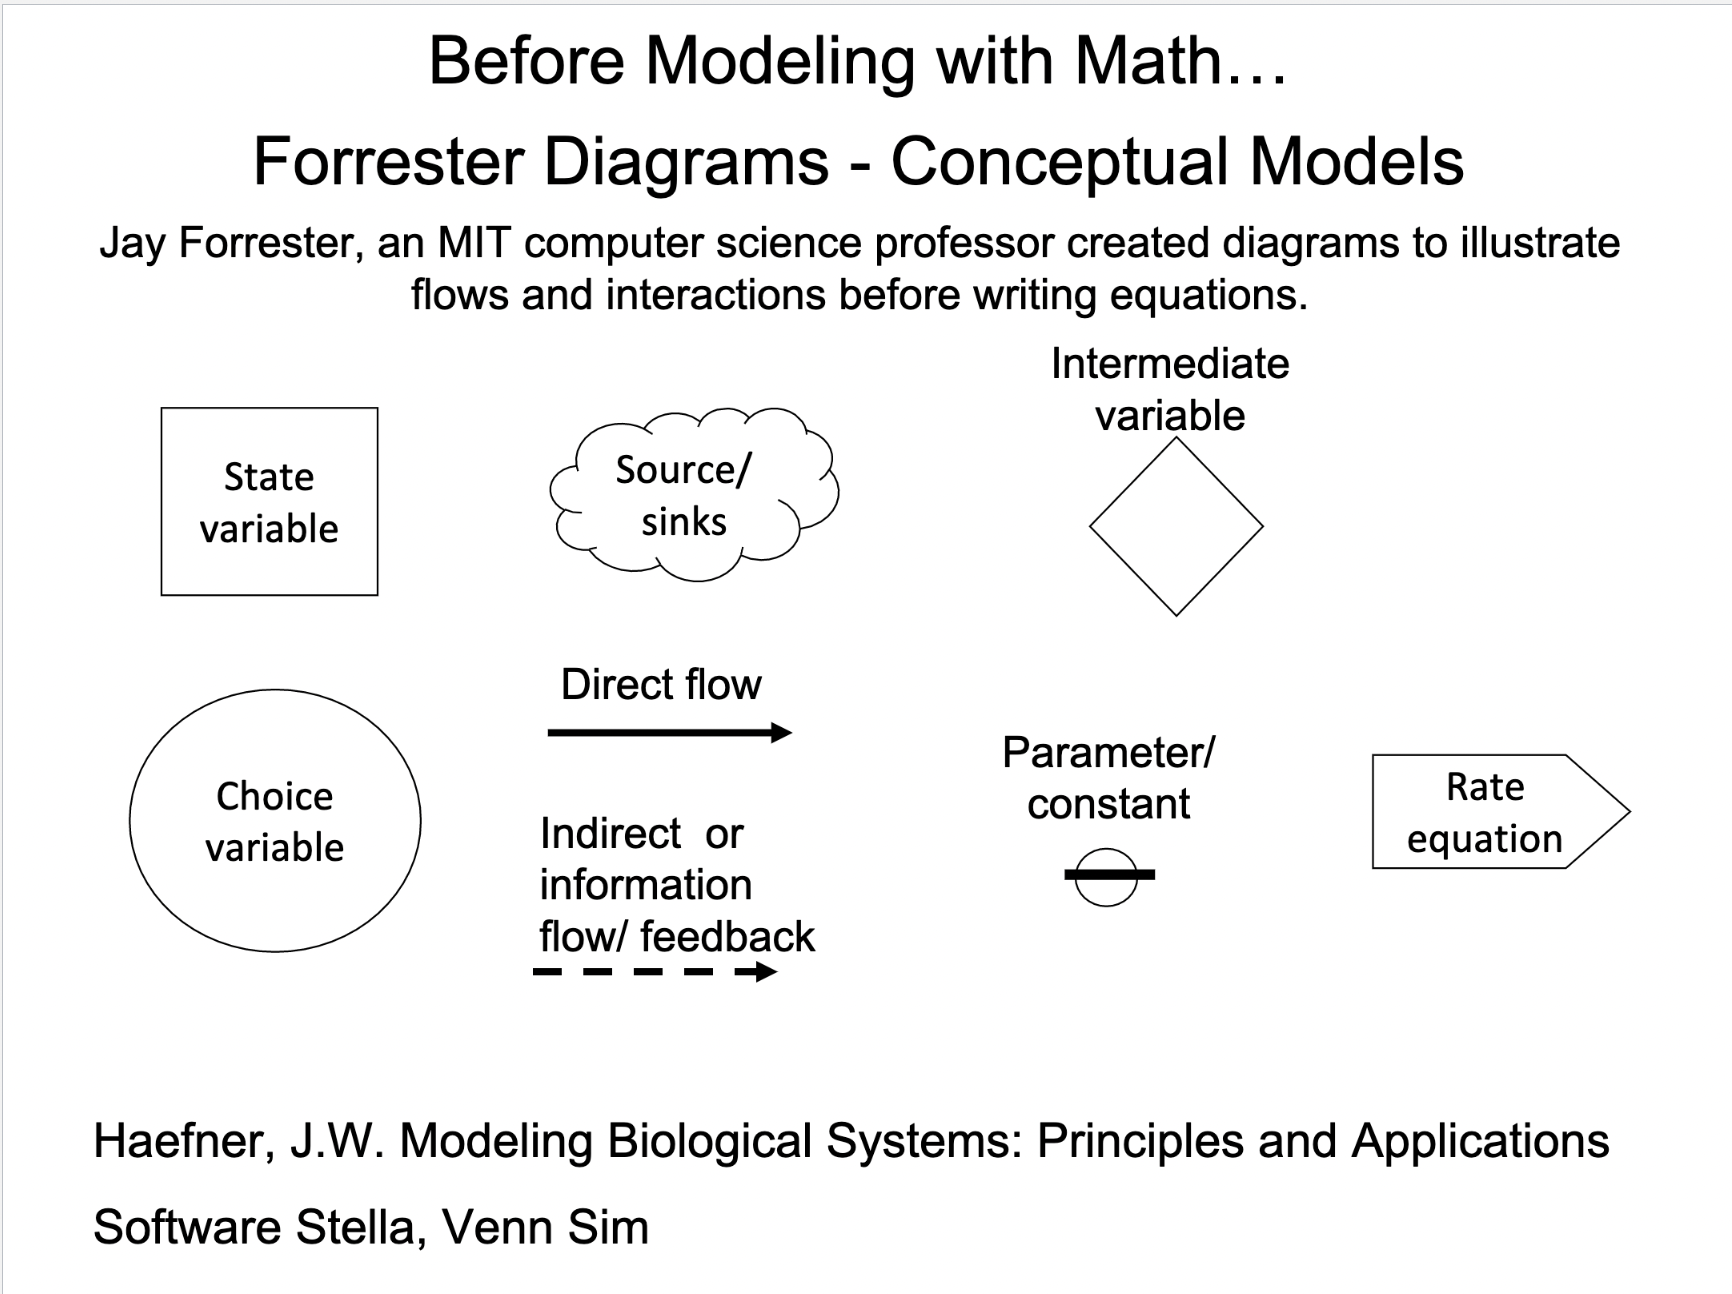
\includegraphics[width=17cm]{forrester_diagrams.png}
        \caption{}
    \end{figure}


\subsection{Review}

\begin{itemize}
    \item Capital is how we store wealth through time 
    \item Durability: everything has a shelf life, so how we value a stock depends on how fast it depreciates 
    \item Ex. Yale decided buying a computer was not a capital investment because computers become outdated so fast 
\end{itemize}


\section{Conceptual Models -- 2/1/23}
Models are an excellent way to make sure a team is on the same page and you can build consensus with that groups. 

\begin{itemize}
    \item State: the quantity of your capital stock of interest
    \item Sources and sinks are boundaries of the system. Where things appear from and where things disappear to. The limit of what we're going to concern ourselves with and what we won't. 
    \item Ex. Climate change has been held outside of economic models for the last 50 years. Was not in the boundaries of the traditional macroeconomic model 
    \item rate equation: birth, death, immigration, emigration 
    \item parameter: some value we assign to something. Something we may try to estimate in order to "parameterize" the system.
    \item flows: both direct and indirect
    \item choice/control variable: what a manager has control over. Typically will be a function of the state
    
\end{itemize}












\end{document}
